\documentclass[aps,prl,reprint,twocolumn,superscriptaddress,nofootinbib,floatfix]{revtex4-2}

\usepackage[utf8]{inputenc}
\usepackage[T1]{fontenc}
\usepackage{amsmath,amssymb,amsfonts,mathtools}
\usepackage{graphicx}
\usepackage{microtype}
\usepackage{booktabs}
\usepackage{enumitem}
\usepackage[dvipsnames]{xcolor}
\usepackage{silence}
\WarningFilter{nameref}{The definition of \label has changed!}
\usepackage{hyperref}

\hypersetup{
  colorlinks=true,
  linkcolor=NavyBlue,
  citecolor=Mahogany,
  urlcolor=TealBlue
}

\providecommand{\R}{\mathbb{R}}
\newcommand{\C}{\mathbb{C}}
\providecommand{\Sph}{\mathbb{S}}
\newcommand{\Tr}{\operatorname{Tr}}
\newcommand{\dif}{\,\mathrm{d}}
\providecommand{\Area}{\operatorname{Area}}
\newcommand{\norm}[1]{\left\|#1\right\|}
\DeclareMathOperator*{\argmin}{argmin}
\providecommand{\Hyp}{\mathbb{H}}
\providecommand{\II}{\mathrm{II}}
\providecommand{\Hsn}{\mathcal{H}}
\providecommand{\BV}{\mathrm{BV}}
\providecommand{\TV}{\mathrm{TV}}
\providecommand{\cutnorm}[1]{\|#1\|_{\square}}
\providecommand{\doi}[1]{\href{https://doi.org/#1}{\nolinkurl{doi:#1}}}

\begin{document}

\title{Observational Signatures of a Running Spectral Dimension:\texorpdfstring{\\}{ }Parametrization and Order-of-Magnitude Assessment}

\author{Reinaldo Maia Silva-Filho}
\email{reinaldo.filho1@estudante.ufla.br}
\affiliation{Programa de P\'os-Gradua\c{c}\~ao em Estat\'istica e Experimenta\c{c}\~ao Agropecu\'aria (PPGEE/DES), Universidade Federal de Lavras (UFLA), Lavras, MG, Brazil}

\date{\today}

\begin{abstract}
A spectral dimension that runs from $d_s = 4$ at large scales to $d_s = 2$ at short scales appears in several approaches to quantum gravity. For the Euclidean heat kernel of the assumed two-scale symbol $k^2 + \ell^2 k^4$ in four dimensions, with $\ell$ a free length, we give its diagonal and $d_s(\tau)$ in closed form, and verify both against numerical quadrature. We then examine four phenomenological ans\"atze discussed in the companion chapters, none of which follows from the heat-kernel model: (i) a quartic correction to the graviton dispersion relation, $\omega^2 = c^2k^2(1 + \xi\ell_\ast^2 k^2)$; (ii) a running of the primordial tensor tilt postulated to track the spectral dimension, $\alpha_t = \frac{1}{2}(d_s - 4)$; (iii) analog measurements in quantum simulators; and (iv) atom interferometry. With $\ell_\ast = \ell_P$, the arrival-time delay between $10$\,Hz and $1$\,kHz for sources at redshifts $1$--$8$ is $\sim 10^{-61}$--$10^{-60}$\,s. Evaluated at the physical momentum of the tensor modes at horizon exit, the tilt running for $M_\ast = M_P$ is $|\alpha_t| \approx (H_{\mathrm{inf}}/M_P)^2 \lesssim 10^{-11}$. Both are many orders of magnitude below experimental reach. In the anisotropic $z = 3$ realization the scale $M_\ast$ cannot be the Planck mass, and we quote the bounds that apply to it. A detectable dispersion delay would require $\ell_\ast \sim 3\times 10^{-7}$\,m, a scale not motivated by the model. Analog simulators and atom interferometers do not test the framework without further input. The purpose of this chapter is to record these estimates explicitly, so that the observational status of the framework is clear.
\end{abstract}

\maketitle

\emph{Introduction.}---The Planck scale $M_P = \sqrt{\hbar c / G} \approx 1.22 \times 10^{19}$\,GeV lies far beyond direct experimental reach, and perturbative quantum general relativity is non-renormalizable \cite{goroff1986ultraviolet}. Proposed signatures of quantum gravity must therefore rely on effects that accumulate over large distances or that are enhanced by some mechanism.

The companion chapters \cite{silvafilho2026grand} discuss a framework combining continuous tensor networks \cite{silvafilho2026functional, silvafilho2026flows, silvafilho2026spacetime}, fractional calculus on continuous Pascal simplices \cite{silvafilho2026pascal}, and $L^\infty$-minimax extrinsic curvature \cite{silvafilho2026noneuclidean}. Chapter~12 records a closed form for the spectral dimension of a heat kernel with an assumed two-scale symbol, an elementary integral. Here we ask which observational signatures could be associated with it, and how large they are.

\begin{figure*}[t]
\centering
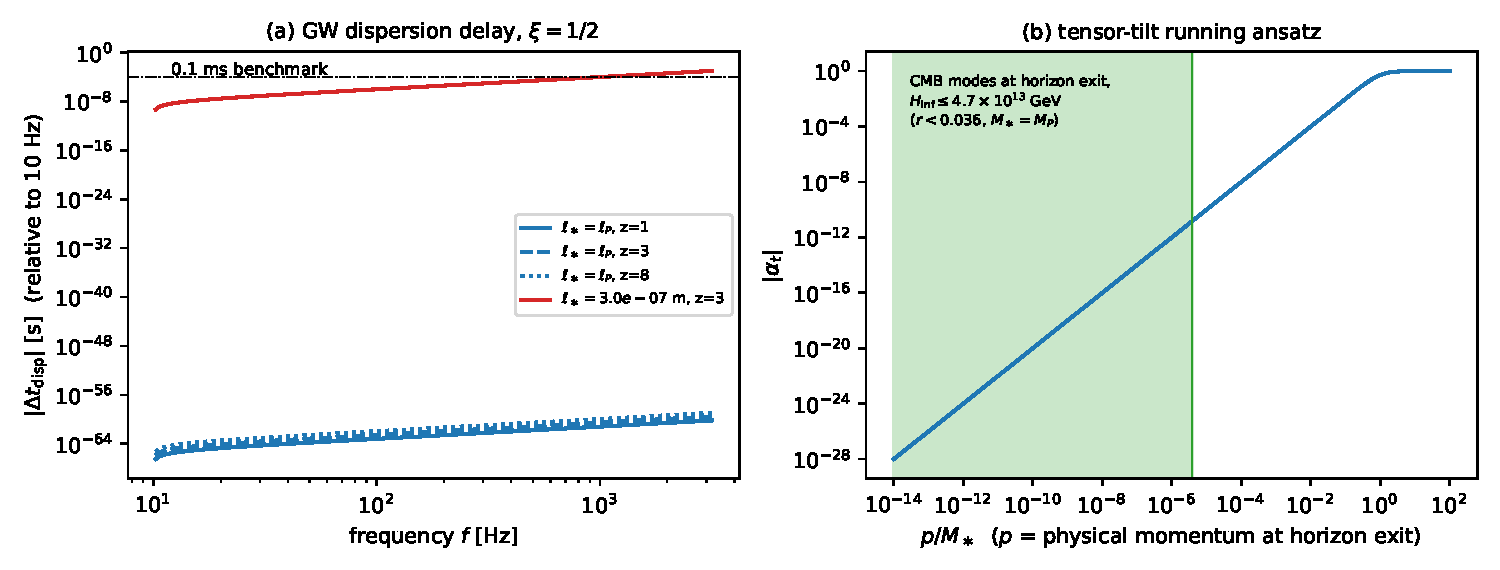
\includegraphics[width=\textwidth]{fig_experimental_signatures.pdf}
\caption{\textbf{Order-of-magnitude assessment.} (a) Arrival-time delay $|\Delta t_{\mathrm{disp}}|$ relative to $10$\,Hz, Eq.~\eqref{eq:delta_t} with $\xi = 1/2$. Blue: $\ell_\ast = \ell_P$ at redshifts $1, 3, 8$, a reference value outside the weak-coupling window of the $z = 3$ Ho\v{r}ava--Lifshitz branch. Red: the value $\ell_\ast \approx 3.0 \times 10^{-7}$\,m that would be required to reach a $0.1$\,ms delay at $1$\,kHz for redshift $3$. Dash-dotted: $0.1$\,ms timing benchmark. (b) The tilt-running ansatz \eqref{eq:tensor_running} as a function of $p/M_\ast$, with $p$ the physical momentum of the mode at horizon exit. The shaded region, $p = H_{\mathrm{inf}} \le 4.71 \times 10^{13}$\,GeV, contains the CMB modes for $M_\ast = M_P$ and $r < 0.036$. The script that generates the figure is in the accompanying code repository.}
\label{fig:experimental}
\end{figure*}

\emph{Running spectral dimension.}---The heat kernel of the isotropic symbol $k^2 + \ell^2 k^4$ (not a positive kernel, hence not a diffusion in the probabilistic sense) in four Euclidean dimensions interpolates between the Laplacian at large scales and the bi-Laplacian at short scales, so $d_s$ runs from $4$ to $4/2 = 2$. The symbol is assumed, with $\ell > 0$ a free length and $\ell_P$ only a reference value: no translation-invariant operator with non-negative jump kernel and non-negative potential, and no continuous refinement limit of such operators, has it \cite{silvafilho2026grand}. The same end values occur in Causal Dynamical Triangulations \cite{ambjorn2005spectral}. In Ho\v{r}ava--Lifshitz gravity they arise from a different, anisotropic operator: with scaling exponent $z$ in $3+1$ dimensions the ultraviolet value is $d_s = 1 + 3/z$, so $d_s = 2$ needs $z = 3$, while $z = 2$ (a spatial $k^4$ term) gives $5/2$ \cite{horava2009spectral}. In $2+1$ dimensions, Sotiriou, Visser and Weinfurtner showed that Ho\v{r}ava--Lifshitz-type dispersion relations reproduce the CDT flow of $d_s$ \cite{sotiriou2011spectral}. Writing $u = k^2$ and $z \coloneqq \sqrt{\tau}/(2\ell)$, its diagonal is
\begin{align}
    \label{eq:heat_kernel_exact}
    P(\tau) &= \frac{1}{16\pi^2} \int_0^\infty u\, e^{-\tau u - \tau \ell^2 u^2} \dif u \nonumber \\
    &= \frac{1}{32\pi^2 \ell^2 \tau} \Big[ 1 - \sqrt{\pi}\, z\, e^{z^2} \operatorname{erfc}(z) \Big],
\end{align}
and $d_s(\tau) \coloneqq -2\, \dif \ln P / \dif \ln \tau$ evaluates to
\begin{equation}
    \label{eq:ds_tau}
    d_s(\tau) = 1 - \frac{\tau}{2\ell^2} + \left[ 1 - \frac{\sqrt{\pi \tau}}{2\ell} e^{\tau/4\ell^2} \operatorname{erfc}\!\left( \frac{\sqrt{\tau}}{2\ell} \right) \right]^{-1}.
\end{equation}
Using $\operatorname{erfc}(z) = 1 - 2z/\sqrt{\pi} + \mathcal{O}(z^3)$ as $z \to 0$ and $\sqrt{\pi}\, z\, e^{z^2} \operatorname{erfc}(z) = 1 - 1/(2z^2) + 3/(4z^4) + \mathcal{O}(z^{-6})$ as $z \to \infty$,
\begin{equation}
    \label{eq:ds_limits}
    \lim_{\tau \to 0} d_s(\tau) = 2, \qquad \lim_{\tau \to \infty} d_s(\tau) = 4.
\end{equation}
In the infrared limit the explicit $-2z^2$ term cancels against the $2z^2 + 3 + \mathcal{O}(z^{-2})$ tail of the reciprocal bracket, and $d_s = 4 - 12\ell^2/\tau + \mathcal{O}(\ell^4/\tau^2)$. Eqs.~\eqref{eq:heat_kernel_exact} and \eqref{eq:ds_tau} agree with direct numerical quadrature to better than $10^{-6}$ for $\tau/\ell^2 \in [10^{-3}, 10^2]$.

\emph{Graviton dispersion.}---The running of $d_s$ does not by itself fix a dispersion relation for gravitational waves. As a phenomenological ansatz, we consider
\begin{equation}
    \label{eq:dispersion}
    \omega^2(k) = c^2 k^2 \left( 1 + \xi \ell_\ast^2 k^2 \right),
\end{equation}
where the heat-kernel model sets no Lorentzian scale and fixes neither $\ell_\ast$ nor $\xi$. Continued to Lorentzian signature, the isotropic symbol $p^2(1 + \ell^2 p^2)$ vanishes on $p^2 = 0$, a massless branch without dispersion ($\xi = 0$), and on $p^2 = -1/\ell^2$, a massive mode with residue $-1$, i.e.\ a ghost \cite{stelle1977renormalization}. The anisotropic operator $\omega^2 + c^2(k^2 + \ell^2 k^4)$, which would give $\xi = 1$, has $d_s \to 5/2$ rather than $2$ in the ultraviolet. A quartic term with $\xi \neq 0$ reaches $d_s \to 2$ in the ultraviolet only inside a $z = 3$ theory with an additional $k^6$ term, where $\xi$ is then an independent coupling; any $\xi \neq 0$ presupposes a preferred frame, and $v_g > c$ for $\xi > 0$ (for $\xi < 0$, $v_g < c$). In the healthy, non-projectable $z = 3$ extension of Ho\v{r}ava--Lifshitz gravity, weak coupling requires $M_\ast \lesssim 10^{15}$--$10^{16}$\,GeV \cite{blas2011models}, so that $M_\ast$ cannot be the Planck mass, and protecting matter from Lorentz violation suggests $M_\ast \lesssim 10^{10}$\,GeV \cite{pospelov2012lorentz}, i.e.\ $\ell_\ast \gtrsim 10^{3}$--$10^{9}\,\ell_P$ in that branch. We treat $\xi$ as a free parameter of order unity; all delays are linear in $\xi$, and we display $\xi = 1/2$. The group velocity is $v_g \approx c(1 + \frac{3}{2}\xi \ell_\ast^2 k^2)$. A graviton observed at frequency $f$ had physical wavenumber $2\pi f (1+z')/c$ at redshift $z'$, so the velocity excess is weighted by $(1+z')^2$ along the path \cite{jacob2008lorentz, mirshekari2012constraining}. Two frequencies emitted together at redshift $z$ therefore arrive separated by
\begin{equation}
    \label{eq:delta_t}
    |\Delta t_{\mathrm{disp}}| = \frac{6 \pi^2 \xi \ell_\ast^2}{c^3} D_2(z) \left( f_2^2 - f_1^2 \right),
\end{equation}
with $D_2(z) = \frac{c}{H_0} \int_0^z \frac{(1+z')^2\,\dif z'}{\sqrt{\Omega_m(1+z')^3 + \Omega_\Lambda}}$.
For $\ell_\ast = \ell_P$, $\xi = 1/2$, $f_1 = 10$\,Hz, $f_2 = 1$\,kHz and $H_0 = 70$\,km\,s$^{-1}$\,Mpc$^{-1}$, $\Omega_m = 0.3$, one finds $|\Delta t_{\mathrm{disp}}| = 6 \times 10^{-62}$, $3 \times 10^{-61}$ and $1.2 \times 10^{-60}$\,s at redshifts $1, 3, 8$ [Fig.~\ref{fig:experimental}(a)]. As a benchmark for third-generation detectors such as the Einstein Telescope \cite{punturo2010einstein} and Cosmic Explorer \cite{reitze2019cosmic} we take a timing accuracy of $10^{-4}$\,s, an optimistic figure corresponding to a phase accuracy of $\sim 0.1$\,rad at $\sim 100$\,Hz for loud events; actual dispersion tests fit the waveform phase rather than arrival times~\cite{ligo2019tgr}. The Planck-scale signal is therefore $56$--$57$ orders of magnitude below this benchmark, and LISA \cite{amaro2017laser}, which observes millihertz frequencies, is less sensitive to an $f^2$ effect; this figure is specific to $\ell_\ast = \ell_P$, which lies outside the weak-coupling window of the $z = 3$ branch. For $\ell_\ast = \hbar c/(10^{10}\,\mathrm{GeV})$, the value suggested by the Lorentz-violation bound of the $z = 3$ branch if the quartic term is not shared by matter fields, as in the scale-separation scenario of \cite{pospelov2012lorentz}, the delays scale by $(\ell_\ast/\ell_P)^2 \approx 1.5 \times 10^{18}$, to $\sim 10^{-43}$--$10^{-42}$\,s, still some $38$ orders of magnitude below the benchmark. A $10^{-4}$\,s delay at redshift $3$ would require $\ell_\ast \approx 3.0 \times 10^{-7}$\,m, an energy scale $\hbar c/\ell_\ast \approx 0.7$\,eV, and nothing in the framework points to such a scale. Read in a preferred frame, the quartic ansatz is weakly constrained by gravitational waves alone: the superluminal side of the GW170817 speed bound gives $\ell_\ast < 1.0 \times 10^{-2}$\,m for $\xi = 1$ \cite{abbott2017gw170817}, and the dispersion test of GWTC-3, $A_4 < 0.30 \times 10^4$\,eV$^{-2}$ for $A_4 > 0$, gives $\ell_\ast < 1.1 \times 10^{-5}$\,m for $\xi = 1$ \cite{gwtc3tgr}. If the same quartic term acts on photons, superluminal photon bounds are far stronger: the LHAASO observation of GRB~221009A gives $E_{\mathrm{QG},2} > 7.0 \times 10^{11}$\,GeV \cite{lhaaso2024}, and photon splitting in the Crab Nebula spectrum gives $\hbar c/\ell_\ast > 4.1 \times 10^{14}$\,GeV, i.e.\ $\ell_\ast < 4.82 \times 10^{-31}$\,m, for $\xi = 1$ \cite{satunin2019}. These photon bounds rest on that universality assumption, which neither quadratic gravity nor Ho\v{r}ava--Lifshitz gravity implies.

\emph{Tensor-tilt running.}---In single-field slow-roll inflation, $\mathcal{P}_t(k) = A_t (k/k_*)^{n_t}$ with $n_t = -r/8$. A two-point Pad\'e form with the limits \eqref{eq:ds_limits} and an infrared approach of the same power as Eq.~\eqref{eq:ds_tau} (the coefficient depends on the identification $\tau \sim p^{-2}$ and is not matched) is $d_s(p) = 2 + 2/(1 + (p/M_\ast)^2)$. If one \emph{postulates} that the running of the tilt tracks the spectral dimension,
\begin{equation}
    \label{eq:tensor_running}
    \alpha_t \coloneqq \frac{\dif n_t}{\dif \ln k} = \frac{1}{2} \left( d_s(p) - 4 \right) = -\frac{(p/M_\ast)^2}{1 + (p/M_\ast)^2},
\end{equation}
the momentum $p$ must be a physical one. A local effect with scale $M_\ast$ acts on a tensor mode when the mode is generated, at horizon exit, where its physical momentum is $p = k/a = H_{\mathrm{inf}}$; the comoving wavenumber measured today depends on the normalization of the scale factor and is not an invariant scale. The bound $r < 0.036$ \cite{bicepkeck2021constraints} and $A_s \approx 2.1 \times 10^{-9}$ \cite{planck2018parameters} give, through $2H_{\mathrm{inf}}^2/(\pi^2 M_{\mathrm{red}}^2) = rA_s$ with $M_{\mathrm{red}} = M_P/\sqrt{8\pi}$, the bound $H_{\mathrm{inf}} \le 4.71 \times 10^{13}$\,GeV. For $M_\ast = M_P$ the running is then $|\alpha_t| \approx (H_{\mathrm{inf}}/M_P)^2 \le 1.5 \times 10^{-11}$ ($3.74 \times 10^{-10}$ for $M_\ast = M_{\mathrm{red}}$), nearly the same for all CMB multipoles because $H_{\mathrm{inf}}$ changes little while they exit the horizon [Fig.~\ref{fig:experimental}(b)]. LiteBIRD \cite{hazumi2019litebird} and CMB-S4 \cite{abazajian2016cmb} target the tensor amplitude at the level $r \sim 10^{-3}$; for $M_\ast = M_P$ a running of $10^{-11}$ in the tensor tilt is far beyond their reach, and the ansatz predicts no observable modification of $C_\ell^{BB}$. For $M_\ast < M_P$ it gives $|\alpha_t| = x/(1+x)$, $x = (H_{\mathrm{inf}}/M_\ast)^2$, which saturates to $1$ as $M_\ast \to 0$; since $H_{\mathrm{inf}}$ is only bounded above, the values that follow are upper bounds. In a $z = 3$ realization, if the quartic term is universal with unit coefficient, photon dispersion bounds leave the window $4.1\times10^{14} \lesssim M_\ast \lesssim 10^{15}$--$10^{16}$\,GeV, where $|\alpha_t|$ is at most of order $10^{-2}$; for $M_\ast \sim 10^{10}$\,GeV it is at most of order one. No cited source establishes whether a shift of this size would be observable.

\emph{Quantum simulators.}---Programmable Rydberg arrays \cite{ebadi2021quantum} and superconducting processors can prepare tensor-network states, estimate their quantum Fisher metrics, and measure out-of-time-order correlators $F(t) = \langle W(t) V(0) W(t) V(0) \rangle_\beta$. The Lyapunov exponent obeys the Maldacena--Shenker--Stanford bound $\lambda_L \le 2\pi k_B T/\hbar$ \cite{maldacena2016bound}, which the SYK model approaches only at strong coupling. Such experiments probe the specific many-body systems realized. They would test the framework only if a concrete model were identified in which its conjectured relations (Conjecture~7.1 of \cite{silvafilho2026grand}) make a quantitative prediction. We do not have such a model.

\begin{table*}[t]
\centering
\caption{\textbf{Summary of the order-of-magnitude assessment} ($\ell_\ast = \ell_P$, $M_\ast = M_P$ unless stated).}
\label{tab:experiments}
\begin{ruledtabular}
\begin{tabular}{lllll}
\textbf{Frontier} & \parbox[t]{2.0cm}{\raggedright\small\textbf{Observable}} & \textbf{Model value} & \parbox[t]{2.0cm}{\raggedright\small\textbf{Instrument reach}} & \parbox[t]{2.5cm}{\raggedright\textbf{Status}} \\
\midrule
Gravitational waves & \parbox[t]{1.9cm}{\raggedright $|\Delta t_{\mathrm{disp}}|$, $10$\,Hz--$1$\,kHz, redshift $1$--$8$} & $10^{-61}$--$10^{-60}$\,s & \parbox[t]{1.9cm}{\raggedright ET, CE: $10^{-4}$\,s (benchmark)} & \parbox[t]{2.5cm}{\raggedright $56$--$57$ orders below reach} \\
\addlinespace[3pt]
CMB & \parbox[t]{1.9cm}{\raggedright tilt running $\alpha_t$ at horizon exit} & $|\alpha_t| \lesssim 10^{-11}$ & \parbox[t]{1.9cm}{\raggedright LiteBIRD, CMB-S4: $r \sim 10^{-3}$} & \parbox[t]{2.5cm}{\raggedright unobservable for $M_\ast = M_P$} \\
\addlinespace[3pt]
Quantum simulators & \parbox[t]{1.9cm}{\raggedright Fisher metric, OTOC} & \parbox[t]{2.1cm}{\raggedright no model-specific prediction} & \parbox[t]{1.9cm}{\raggedright Rydberg arrays, transmons} & \parbox[t]{2.5cm}{\raggedright requires a concrete model} \\
\addlinespace[3pt]
Atom interferometry & \parbox[t]{1.9cm}{\raggedright $\ell_P/\lambda_{\mathrm{dB}}$, Sr, $v \lesssim 45$\,m/s} & $\lesssim 2 \times 10^{-25}$ & \parbox[t]{1.9cm}{\raggedright MAGIS-100, AION} & \parbox[t]{2.5cm}{\raggedright no test proposed} \\
\end{tabular}
\end{ruledtabular}
\end{table*}

\emph{Atom interferometry.}---Long-baseline atom interferometers (MAGIS-100 \cite{abe2021matter}, AION \cite{badurina2020aion}) do not test a ``Jordan-loop protection'' of loop-quantum-gravity holonomies. Such a test would require the restriction to non-self-intersecting loops to follow from chronology protection. Chronology constrains timelike curves, whereas the loops in question are spacelike, and the restriction is a conjecture about a kinematical sector (Conjecture~4.3 of \cite{silvafilho2026grand}). Moreover, for $^{87}$Sr atoms $\ell_P/\lambda_{\mathrm{dB}} = m v \ell_P/(2\pi\hbar) \approx 3.5 \times 10^{-27}\,(v/1\,\mathrm{m\,s^{-1}})$, which stays below $2 \times 10^{-25}$ for the launch velocities ($v \lesssim 45$\,m\,s$^{-1}$) of long-baseline instruments; no prediction of the framework is attached to this ratio.

\emph{Conclusion.}---The closed form \eqref{eq:ds_tau} gives an explicit, numerically verified interpolation of the spectral dimension between $2$ and $4$ for a two-scale heat kernel. The observational ans\"atze associated with it, with the scale set by $\ell_P$, give effects suppressed by factors of order $(\ell_P k)^2$ for gravitational waves and $(H_{\mathrm{inf}}/M_P)^2$ for the tensor tilt, far below the reach of gravitational-wave and CMB experiments. In the anisotropic $z = 3$ realization with $d_s = 2$ the scale is not $\ell_P$, and the bounds above apply to it. For quantum simulators and atom interferometers the framework makes no prediction to compare with. The framework in its present form makes no observable prediction. Obtaining one would require an independent mechanism that enhances Planck-suppressed effects, or a lower scale $\ell_\ast$ justified from first principles.

\begin{acknowledgments}
This research was financed in part by the Coordena\c{c}\~ao de Aperfei\c{c}oamento de Pessoal de N\'ivel Superior -- Brasil (CAPES) -- Finance Code 001. The author thanks the faculty and researchers at UFLA PPGEE/DES for institutional support and valuable discussions.
\end{acknowledgments}

% Shared declarations block: the single source for the declarations of the book.
% \input by every standalone chapter before its bibliography, and \input ONCE in the
% front matter of the single-source master (official_master_structure.tex); the
% chapter bodies of the master do not repeat it (extract.py drops their \input).
% \gtqgdeclscope is "chapter" by default; the master sets it to "book" before \input.
% Aligned with the Leiden Declaration on Artificial Intelligence and Mathematics
% (arXiv:2609.35334); see _staging/DECLARACOES_IA_PROPOSTA.md Sec.4.2 for the rationale.
\providecommand{\gtqgdeclscope}{chapter}
\section*{Declarations}

\noindent\textbf{Funding.} This research was financed in part by the Coordena\c{c}\~ao de Aperfei\c{c}oamento de Pessoal de N\'ivel Superior -- Brasil (CAPES) -- Finance Code 001.

\medskip\noindent\textbf{Competing interests.} The author declares no competing interests.

\medskip\noindent\textbf{Tool and computational resource disclosure.} In line with the Leiden Declaration on Artificial Intelligence and Mathematics (arXiv:2609.35334), the author discloses that large language model assistants (Anthropic Claude; Google Gemini, used through the Antigravity agent environment) were used extensively in preparing this work: drafting and editing text and \LaTeX{} source; proposing, expanding and revising derivations and proofs under the author's direction; writing the Python verification scripts and the \textsc{Lean 4} files; searching and checking the literature and references; and adversarial auditing of proofs, numerical claims and code. These audits found errors, some of them originally introduced with AI assistance; the errors and their corrections are recorded in \texttt{WORKPLAN.md}. Where a result builds on a specific prior idea, the author has sought to identify and cite its source, and states explicitly where a satisfactory attribution could not be established.

\medskip\noindent\textbf{Authorship and responsibility.} AI tools are not authors of this work. Credit and responsibility for its content belong solely to the human author, who chose the research questions and the overall framework, reviewed the material, and is responsible for the content, including any remaining errors.

\medskip\noindent\textbf{Verification status.} Results labelled Theorem, Proposition or Lemma are proved in the text or cited as classical; statements labelled Conjecture are not proved. The numerical scripts compare formulas of the text with independent computations and are checks, not proofs. The \textsc{Lean 4} modules in \texttt{formal\_proofs\_book/Book} are a naming skeleton and do not verify the mathematics of this \gtqgdeclscope; they do not constitute the formal verification the Leiden Declaration asks organisations to consider for automated results. Selected results of Chapters~1--13 are formalized in \textsc{Lean 4} with Mathlib in the repository folder \texttt{formal\_proofs\_mathlib}, at the level stated there (in several cases a declared special case); in particular, the Chapter~12 constraint bounds are formalized in a matrix-level form with the ADM constraint taken as a hypothesis, the Chapter~8 curvature identities only in their pointwise algebraic part, with the Gauss, Raychaudhuri and Einstein equations they use taken as hypotheses, and the Chapter~8 U-turn and causal statements in the reduced forms stated there, the Chapter~11 minimum-cut entanglement-entropy bound only in its linear-algebra half, with the tensor-network factorization taken as a hypothesis, together with the inequality $g^{\mathrm{BKM}} \geq g^{\mathrm{SLD}}$ for full-rank $\rho_0$ in its eigenbasis, and the Chapter~13 closed-form running spectral dimension and tensor-tilt arithmetic with the bracket-nonzero hypothesis of that formula left unproved (true on the whole domain by Mills' inequality, not formalized) and the CODATA inputs taken as data. The same folder also covers selected results of the \textit{Simplicial Quantum Gravity}, Yang--Mills, fermion-mass, \textit{Beyond the Spectrum} and \textit{Functorial Bridge} companion works.

\medskip\noindent\textbf{Publication status.} This monograph is distributed as a preprint on Zenodo under the CC~BY~4.0 license. It has not yet been through peer review; Zenodo is a repository, not a peer-reviewed venue.

\medskip\noindent\textbf{Code and data availability.} Sources, numerical scripts and the audit log are available at
\begin{center}\url{https://github.com/reinaldomsilvafilho-netizen/quantum-gravity-lean4}.\end{center}
The monograph is archived on Zenodo, \href{https://doi.org/10.5281/zenodo.22290043}{doi:10.5281/zenodo.22290043}, under the CC~BY~4.0 license.


\begin{thebibliography}{99}

\bibitem{abbott2017gw170817}
B.~P. Abbott et~al. (LIGO Scientific Collaboration, Virgo Collaboration, Fermi GBM, INTEGRAL),
\emph{Gravitational waves and gamma-rays from a binary neutron star merger: GW170817 and GRB 170817A},
Astrophys. J. Lett., \textbf{848} (2017), L13,
\doi{10.3847/2041-8213/aa920c}.

\bibitem{ligo2019tgr}
B.~P.~Abbott et~al. (LIGO Scientific Collaboration and Virgo Collaboration),
\emph{Tests of general relativity with the binary black hole signals from the LIGO-Virgo catalog GWTC-1},
Phys. Rev. D, \textbf{100} (2019), 104036,
\href{https://doi.org/10.1103/PhysRevD.100.104036}{doi:10.1103/PhysRevD.100.104036}.

\bibitem{horava2009spectral}
P.~Ho\v{r}ava,
\emph{Spectral dimension of the universe in quantum gravity at a Lifshitz point},
Phys. Rev. Lett., \textbf{102} (2009), 161301,
\doi{10.1103/PhysRevLett.102.161301}.

\bibitem{sotiriou2011spectral}
T.~P. Sotiriou, M.~Visser, and S.~Weinfurtner,
\emph{Spectral dimension as a probe of the ultraviolet continuum regime of causal dynamical triangulations},
Phys. Rev. Lett., \textbf{107} (2011), 131303,
\doi{10.1103/PhysRevLett.107.131303}.

\bibitem{blas2011models}
D.~Blas, O.~Pujol\`as, and S.~Sibiryakov,
\emph{Models of non-relativistic quantum gravity: the good, the bad and the healthy},
JHEP, \textbf{2011} (2011), no.~4, 018,
\doi{10.1007/JHEP04(2011)018}.

\bibitem{pospelov2012lorentz}
M.~Pospelov and Y.~Shang,
\emph{Lorentz violation in Ho\v{r}ava--Lifshitz-type theories},
Phys. Rev. D, \textbf{85} (2012), 105001,
\doi{10.1103/PhysRevD.85.105001}.

\bibitem{stelle1977renormalization}
K.~S. Stelle,
\emph{Renormalization of higher-derivative quantum gravity},
Phys. Rev. D, \textbf{16} (1977), 953--969,
\doi{10.1103/PhysRevD.16.953}.

\bibitem{gwtc3tgr}
R.~Abbott et~al. (LIGO Scientific, Virgo and KAGRA Collaborations),
\emph{Tests of general relativity with GWTC-3},
Phys. Rev. D, \textbf{112} (2025), 084080,
\doi{10.1103/PhysRevD.112.084080}.

\bibitem{lhaaso2024}
Z.~Cao et~al. (LHAASO Collaboration),
\emph{Stringent tests of Lorentz invariance violation from LHAASO observations of GRB 221009A},
Phys. Rev. Lett., \textbf{133} (2024), 071501,
\doi{10.1103/PhysRevLett.133.071501}.

\bibitem{satunin2019}
P.~Satunin,
\emph{New constraints on Lorentz invariance violation from Crab Nebula spectrum beyond 100 TeV},
Eur. Phys. J. C, \textbf{79} (2019), 1011,
\doi{10.1140/epjc/s10052-019-7520-y}.

\bibitem{abazajian2016cmb}
K.~N. Abazajian et~al.,
\emph{CMB-S4 Science Book, First Edition},
arXiv:1610.02743 (2016),
\doi{10.48550/arXiv.1610.02743}.

\bibitem{abe2021matter}
M.~Abe et~al.,
\emph{Matter-wave atomic gradiometer interferometric sensor (MAGIS-100)},
Quantum Sci. Technol., \textbf{6} (2021), 044003,
\doi{10.1088/2058-9565/abf719}.

\bibitem{amaro2017laser}
P.~Amaro-Seoane et~al.,
\emph{Laser Interferometer Space Antenna},
arXiv:1702.00786 (2017),
\doi{10.48550/arXiv.1702.00786}.

\bibitem{ambjorn2005spectral}
J.~Ambj{\o}rn, J.~Jurkiewicz, and R.~Loll,
\emph{The spectral dimension of the universe is scale dependent},
Phys. Rev. Lett., \textbf{95} (2005), 171301,
\doi{10.1103/PhysRevLett.95.171301}.

\bibitem{badurina2020aion}
L.~Badurina et~al.,
\emph{AION: An Atom Interferometer Observatory and Network},
J. Cosmol. Astropart. Phys., \textbf{2020} (2020), 011,
\doi{10.1088/1475-7516/2020/05/011}.

\bibitem{ebadi2021quantum}
S.~Ebadi et~al.,
\emph{Quantum phases of matter on a 256-atom programmable quantum simulator},
Nature, \textbf{595} (2021), 227--232,
\doi{10.1038/s41586-021-03582-4}.

\bibitem{goroff1986ultraviolet}
M.~H. Goroff and A.~Sagnotti,
\emph{The ultraviolet behavior of Einstein gravity},
Nuclear Physics B, \textbf{266} (1986), no.~3-4, 709--736,
\doi{10.1016/0550-3213(86)90193-8}.

\bibitem{hazumi2019litebird}
M.~Hazumi et~al.,
\emph{LiteBIRD: A satellite for the studies of B-mode polarization and Inflation from cosmic background radiation detection},
J. Low Temp. Phys., \textbf{194} (2019), 443--452,
\doi{10.1007/s10909-019-02150-5}.

\bibitem{maldacena2016bound}
J.~Maldacena, S.~H. Shenker, and D.~Stanford,
\emph{A bound on chaos},
J. High Energ. Phys., \textbf{2016} (2016), 106,
\doi{10.1007/JHEP08(2016)106}.

\bibitem{punturo2010einstein}
M.~Punturo et~al.,
\emph{The Einstein Telescope: a third-generation gravitational wave observatory},
Class. Quantum Grav., \textbf{27} (2010), 194002,
\doi{10.1088/0264-9381/27/19/194002}.

\bibitem{reitze2019cosmic}
D.~Reitze et~al.,
\emph{Cosmic Explorer: The U.S. contribution to gravitational-wave astronomy beyond LIGO},
Bull. Am. Astron. Soc., \textbf{51} (2019), 035,
\doi{10.48550/arXiv.1907.04833}.

\bibitem{jacob2008lorentz}
U.~Jacob and T.~Piran,
\emph{Lorentz-violation-induced arrival delays of cosmological particles},
J. Cosmol. Astropart. Phys., \textbf{2008} (2008), 031,
\doi{10.1088/1475-7516/2008/01/031}.

\bibitem{mirshekari2012constraining}
S.~Mirshekari, N.~Yunes, and C.~M. Will,
\emph{Constraining Lorentz-violating, modified dispersion relations with gravitational waves},
Phys. Rev. D, \textbf{85} (2012), 024041,
\doi{10.1103/PhysRevD.85.024041}.

\bibitem{bicepkeck2021constraints}
P.~A.~R. Ade et~al. (BICEP/Keck Collaboration),
\emph{Improved constraints on primordial gravitational waves using Planck, WMAP, and BICEP/Keck observations through the 2018 observing season},
Phys. Rev. Lett., \textbf{127} (2021), 151301,
\doi{10.1103/PhysRevLett.127.151301}.

\bibitem{planck2018parameters}
N.~Aghanim et~al. (Planck Collaboration),
\emph{Planck 2018 results. VI. Cosmological parameters},
Astron. Astrophys., \textbf{641} (2020), A6,
\doi{10.1051/0004-6361/201833910}.

\bibitem{silvafilho2026flows} R.~M. Silva-Filho, \emph{Geometric Flows, Partial Differential Equations, and Variational Dynamics on Matrix and Tensor Manifolds}, Chapter~2 of \emph{Geometry, Tensors, and Quantum Gravity}, Universidade Federal de Lavras, 2026.

\bibitem{silvafilho2026functional} R.~M. Silva-Filho, \emph{Functional Realizations of Matrices and Hypertensors: Emergent Invariants and Geometric Measures}, Chapter~1 of \emph{Geometry, Tensors, and Quantum Gravity}, Universidade Federal de Lavras, 2026.

\bibitem{silvafilho2026grand} R.~M. Silva-Filho, \emph{Emergent Spacetime, Holographic Entanglement, and Quantum Geometry: Proved Results, Conjectures, and Observational Limits}, Chapter~12 of \emph{Geometry, Tensors, and Quantum Gravity}, Universidade Federal de Lavras, 2026.

\bibitem{silvafilho2026noneuclidean} R.~M. Silva-Filho, \emph{Minimax Extrinsic Curvature in Non-Euclidean Geometries and General Relativity: Variational Theory, Space Forms, and ADM Spacetime Slicings}, Chapter~8 of \emph{Geometry, Tensors, and Quantum Gravity}, Universidade Federal de Lavras, 2026.

\bibitem{silvafilho2026pascal} R.~M. Silva-Filho, \emph{Analytic Continuation of Pascal's Simplex: Continuous Multinomial Integrals, Polytope Boundary Recurrences, and Simplicial Fractional Calculus}, Chapter~3 of \emph{Geometry, Tensors, and Quantum Gravity}, Universidade Federal de Lavras, 2026.

\bibitem{silvafilho2026spacetime} R.~M. Silva-Filho, \emph{Emergent Spacetime and Quantum Geometry: Tensor Networks, Holonomies, and Entanglement (Established Results and Conjectures)}, Chapter~11 of \emph{Geometry, Tensors, and Quantum Gravity}, Universidade Federal de Lavras, 2026.

\end{thebibliography}

\end{document}
